\documentclass[11pt,a4paper]{article}
% allow both latex and PDFlatex compatibility  (from pdfTeX FAQ)
\usepackage{hyperlatex}

\usepackage{pifont}
\usepackage{amsmath}
\usepackage{amssymb}
%\usepackage{psfig}
\usepackage{array}
\usepackage{supertabular}
%\usepackage{fancyheadings}
%\usepackage{here}
%\usepackage{pslatex}
\usepackage{eepic,epic}
%\usepackage{pslatex}%{\c c}a serait cens{\'e} corriger le pb de fontes dans les pdfs mais le fichier produit est pas beau
\usepackage[english]{babel}
\usepackage{alltt}

\texonly{\usepackage{graphicx}
\usepackage{makeidx}
\usepackage[pdftex,pageanchor=true,hyperindex=true,pagebackref=true,pdfhighlight=/O,pdfauthor={Yves Renard}]{hyperref}%pour le pdf
\usepackage{xspace} % insere un espace si necessaire 
\usepackage{underscore}
 %\usepackage{fancyheadings}
\usepackage{amsmath}
\usepackage{amssymb}
\usepackage{psfig}
\usepackage{here}
\usepackage{array}
\usepackage{alltt}
\usepackage{graphicx}
\usepackage{eepic,epic}
\usepackage[latin1]{inputenc}
\usepackage[T1]{fontenc}
% \usepackage[french]{babel}
% \usepackage[dvips]{epsfig}

%\oddsidemargin -0.2cm
%\evensidemargin -0.2cm
%\topmargin -1cm
%\textheight 22.5cm
%\textwidth 16.2cm
%\headheight 1.0cm

\newfont{\eufmtwelve}   {eufm10 scaled \magstep1}
\newfont{\eufmten}      {eufm10 }
\newfont{\eufmnine}     {eufm9 }
\newfont{\eufmeight}    {eufm8 }
\newfont{\eufmseven}    {eufm7 }
\newfont{\eufmsix}      {eufm6 }
\newfont{\eufmfive}     {eufm5 }
\newfont{\eusmtwelve}   {eusm10 scaled \magstep1}
\newfont{\eusmten}      {eusm10}
\newfont{\eusmnine}     {eusm9 }
\newfont{\eusmeight}    {eusm8 }
\newfont{\eusmseven}    {eusm7 }
\newfont{\eusmsix}      {eusm6 }
\newfont{\eusmfive}     {eusm5 }
\newfont{\msbmtwelve}   {msbm10 scaled \magstep1}
\newfont{\msbmeight}    {msbm8}

\newcommand{\udl}{\underline}
\newcommand{\udll}[1]{{\udl{\udl{#1}}}}
\newcommand{\udlll}[1]{{\udl{\udl{\udl{#1}}}}}
\newcommand{\mat}[1]{{\mbox{\msbmtwelve {#1}}}}
\newcommand{\Reel}{{\mbox{\msbmtwelve R}}}      % L'ensemble des reels.
\newcommand{\reel}{{\mbox{\msbmeight R}}}       % L'ensemble des reels.
%\newcommand{\Reel}{{\rm I\hspace{-0.15em}R}}
\newcommand{\Complex}{\mbox{\msbmtwelve C}}     % L'ensemble des complexes.
\newcommand{\Naturel}{\mbox{\msbmtwelve N}}  % L'ensemble des entiers naturels.
\newcommand{\naturel}{\mbox{\msbmeight N}}   % L'ensemble des entiers naturels.

%\newcommand{\Naturel}{{\rm I\hspace{-0.15em}N}}% L'ensemble des entiers naturels.
\renewcommand{\emptyset}{\mbox{$\circ$\hspace{-.50em}/}}  % ensemble vide.
\newcommand{\Cont}{{\cal C}}            % L'ensemble des fonctions continues
\newcommand{\Cinf}{{\cal C}^{\infty}}   % L'ensemble des fonction C-infinies
\renewcommand{\vec}[1]{\overrightarrow{\!\!#1}}
\newcommand{\subsetcont}{{\subset\hspace{-.6em}_{\scriptscriptstyle >} }}
\newcommand{\Frac}[2]{{\ds \frac{\ds #1}{\ds #2}}}
\newcommand{\interior}[1]{{\stackrel{\circ}{#1}}}
\newcommand{\cqfd}{{$\mbox{}$\hfill\rule{2.5mm}{2.5mm}}}
\newcommand{\vectwo}[2]{{\left(\hspace{-.5em}\begin{array}{c} {#1} \\ {#2}
     \end{array}\hspace{-.5em}\right)}}
\newcommand{\vecthree}[3]{{\left(\hspace{-.5em}\begin{array}{c} {#1}
     \\ {#2} \\ {#3} \end{array}\hspace{-.5em}\right)}}
\newcommand{\vecfour}[4]{{\left(\hspace{-.5em}\begin{array}{c} {#1}
     \\ {#2} \\ {#3} \\ {#4} \end{array}\hspace{-.5em}\right)}}
\newcommand{\vecfive}[5]{{\left(\hspace{-.5em}\begin{array}{c} {#1}
     \\ {#2} \\ {#3} \\ {#4} \\ {#5} \end{array}\hspace{-.5em}\right)}}
\newcommand{\vecseven}[7]{{\left(\hspace{-.5em}\begin{array}{c} {#1}
     \\ {#2} \\ {#3} \\ {#4} \\ {#5} \\ {#6} \\ {#7} \end{array}\hspace{-.5em}\right)}}
\def\infess{\mathop{\iflanguage{english}{\mbox{ess$\,$inf}}{\mbox{inf$\,$ess}}}}
\def\supess{\mathop{\iflanguage{english}{\mbox{ess$\,$sup}}{\mbox{sup$\,$ess}}}}
\def\essinf{\mathop{\iflanguage{english}{\mbox{ess$\,$inf}}{\mbox{inf$\,$ess}}}}
\def\esssup{\mathop{\iflanguage{english}{\mbox{ess$\,$sup}}{\mbox{sup$\,$ess}}}}
\def\aplim{\mathop{\mbox{ap$\,$lim}}}
\def\aplimsup{\mathop{\mbox{ap$\,$lim$\,$sup}}}
\def\apliminf{\mathop{\mbox{ap$\,$lim$\,$inf}}}
\def\convto{\mathop{\hbox{\rightarrowfill}}} % converge vers.
\newcommand{\rightgap}{{]\hspace{-0.12em}]}}
\newcommand{\leftgap}{{[\hspace{-0.12em}[}}
\newcommand{\gapof}[1]{{\leftgap {#1} \rightgap}}
\newcommand{\restrictiona}[1]
{{ \begin{picture}(13,10) \put(-1,-4){$\mid_{#1}$} \end{picture}
}} % Le signe "Restriction sur #1"

\def\Indic{\mbox{1\hspace{-0.20em}I}}   % Fonction l'indicatrice

% \def\bar3{|\hspace{-1pt}\|} % 3bar verticaux pour les normes matricielles.
\def\cvweak{\mathop{-\hspace{-0.3em}-\hspace{-0.6em}\rightharpoonup}} % fleche cv faible
\def\cvweakstar{\cvweak^*} % fleche cv faible etoile
\def\longmapsto
{ \begin{picture}(0,10)
  \put(0,0){$\scriptstyle{\vdash}$} \end{picture} \mbox{$\longrightarrow$}
} 

\def\build#1_#2^#3{\mathrel{
 \mathop{\kern 0pt#1}\limits_{#2}^{#3}}} % Ecrire en dessous et dessus un symbole.

\def\Dist{\mbox{\eusmtwelve D}} %signe de distribution
\def\dist{\mbox{\eusmten D}} %signe de distribution


%definition de commandes utilises
\newcommand{\ds}{\displaystyle}
\newcommand{\rc}{{\par}}
\newcommand{\rcc}{{\par\medskip}}
\newcommand{\rccc}{{\par\bigskip}}


%definition des environnements theoreme, lemme, ...
\usepackage{boxedminipage}
% \newenvironment{largebox}
%   { \rc\noindent \begin{boxedminipage}[t]{\textwidth} }
%   { \end{boxedminipage}  \rccc\noindent }
\newenvironment{largebox}
  { \rc\noindent \begin{boxedminipage}[t]{\linewidth} }
  { \end{boxedminipage}  \rccc\noindent }


\newtheorem{ltheoreme}{Th\'eor\`eme}
\newenvironment{theoreme}
  { \begin{largebox} \begin{ltheoreme} }
  { \end{ltheoreme} \end{largebox} }
\newtheorem{lproposition}{Proposition}
\newenvironment{proposition}
  { \begin{largebox} \begin{lproposition} }
  { \end{lproposition} \end{largebox} }
\newtheorem{llemme}{Lemme}
\newenvironment{lemme}
  { \begin{largebox} \begin{llemme} }
  { \end{llemme} \end{largebox} }
\newtheorem{ldefinition}{D\'efinition}
\newenvironment{definition}
  { \begin{largebox} \begin{ldefinition} }
  { \end{ldefinition} \end{largebox} }
\newtheorem{lhypothese}{Hypoth\`ese}
\newenvironment{hypothese}
  { \begin{largebox} \begin{lhypothese} }
  { \end{lhypothese} \end{largebox} }
\newtheorem{lcorollaire}{Corollaire}
\newenvironment{corollaire}
  { \begin{largebox} \begin{lcorollaire} }
  { \end{lcorollaire} \end{largebox} }
\newenvironment{remarque}
  { \begin{largebox} {\bf \udl{Remarque} : }}
  { \end{largebox} }

\newcounter{numberofprobl}
\setcounter{numberofprobl}{1}

\newlength{\compteurtpourprobla}
\newlength{\compteurtpourproblb}
\newenvironment{caseeqnarray}[1]
  {
   $${#1}
   \settowidth{\compteurtpourprobla}{${#1}\left\{\right.$}
   \setlength{\compteurtpourproblb}{\textwidth}
   \addtolength{\compteurtpourproblb}{-1\compteurtpourprobla}
   \settowidth{\compteurtpourprobla}{$\;$}
   \addtolength{\compteurtpourproblb}{-1\compteurtpourprobla}
   \left\{ \begin{minipage}[l]{\compteurtpourproblb}
   \vspace{-1em} \begin{eqnarray}
  }
  { \end{eqnarray} \end{minipage} \right. $$}


\newtheorem{hypothesis}{Hypothesis}
\newtheorem{prop}{Proposition}
\newtheorem{defi}{Definition}
%\newtheorem{theorem}{Theorem}
%\newtheorem{lemma}{Lemma}


% pour plus tard ...
% \DeclareGraphicsRule{ps.Z}{eps}{ps.bb}{`zcat #1}
% \DeclareGraphicsRule{eps.Z}{eps}{eps.bb}{`zcat #1}
% \DeclareGraphicsRule{ps.gz}{eps}{ps.bb}{`gunzip #1}
% \DeclareGraphicsRule{eps.gz}{eps}{eps.bb}{`gunzip #1}

\newcommand{\ds}{\displaystyle}
\newcommand{\Frac}[2]{{\ds \frac{\ds #1}{\ds #2}}}
\oddsidemargin -0.9cm
\evensidemargin -0.9cm
\topmargin -1cm
\textheight 22.5cm
\textwidth 17.6cm
\headheight 1.0cm
}
\makeindex

% \W .. is equivalent to \htmlonly{..}
\W \newcommand{\HlxIcons}{./}
%\W \usepackage{frames} % navigation panel
\W \htmldirectory{gmmuser}
\W \htmlname{gmmuser}
\W \setcounter{htmldepth}{2}
\W \setcounter{htmlautomenu}{2}
\W \renewcommand{\HlxMeta}{\xml{META description="GMM++ user manual"}}
\htmlonly{
  \htmlpanelfield{Index}{gmmuser}
  \htmlcss{docstyle.css}
  \newcommand{\text}[1]{\mathrm{#1}}
  \newcommand{\WEB}[2]{\xmlattributes*{a}{target="_top"}\xlink{#2}{#1}}
  \newcommand{\nabla}{\htmlsym{nabla}}%renamed \xmlent by lastest version of hyperlatex
  \newcommand{\ell}{\htmlsym{tau}}
  \newcommand{\lambda}{\htmlsym{lambda}}
  \newcommand{\varepsilon}{\htmlsym{epsilon}}
  \newcommand{\phi}{\htmlsym{phi}}
  \newcommand{\varphi}{\htmlsym{phi}}
  \newcommand{\psi}{\htmlsym{psi}}
  \newcommand{\sigma}{\htmlsym{sigma}}
  \newcommand{\nu}{\htmlsym{nu}}
  \newcommand{\beta}{\htmlsym{beta}}
  \newcommand{\gamma}{\htmlsym{gamma}}
  \newcommand{\Gamma}{\htmlsym{Gamma}}
  \newcommand{\Delta}{\htmlsym{Delta}}
  \newcommand{\delta}{\htmlsym{delta}}
  \newcommand{\Omega}{\htmlsym{Omega}}
  \newcommand{\omega}{\htmlsym{omega}}
  \newcommand{\partial}{\htmlsym{part}}
  \newcommand{\sum}{\htmlsym{sum}}
  \newcommand{\int}{{\Large\htmlsym{int}}}
}
\T \newcommand{\Div}{\textrm{div}}
\W \newcommand{\Div}{div}
\T \newcommand{\Grad}{\textrm{grad}}
\W \newcommand{\Grad}{grad}
\T \newcommand{\Rot}{\textrm{curl}}
\W \newcommand{\Rot}{curl}

\W \newcommand{\gmm}{GMM++ }
\T \newcommand{\gmm}{{\sc Gmm++\ }\xspace}

\W \newcommand{\newpage}{}
\W \newcommand{\hspace}[1]{ }
\W \newcommand{\left}{} % pour les left\(i\right) 
\W \newcommand{\right}{}
\W \newenvironment{alltt}{\begin{example}}{\end{example}}
\T \newenvironment{cppcode}{\begin{alltt}}{\end{alltt}}
\W \newenvironment{cppcode}{\begin{rawxml}<div class="cppcode">\end{rawxml}\begin{example}}{\end{example}\begin{rawxml}</div>\end{rawxml}}
\T \newcommand{\cpp}[1]{\texttt{#1}}
\T \newcommand{\filename}[1]{\texttt{#1}}
\W \newcommand{\cpp}[1]{\xmlattributes*{tt}{class="inlinecppcode"}\texttt{#1}}
\W \newcommand{\filename}[1]{\xmlattributes*{tt}{style="color:red"}\texttt{#1}}

\T \newenvironment{ctableau}[2]{\begin{center}\begin{supertabular}{#1}}{\end{supertabular}\end{center}}
\W \newenvironment{ctableau}[2]{\xmlattributes*{table}{border=1 align="center"}\begin{tabular}{#2}}{\end{tabular}}
\begin{document}
\htmltitle{Gmm++ User Guide}
\htmlpanel{0}%disable navigation panel

\begin{center}
\texonly{
  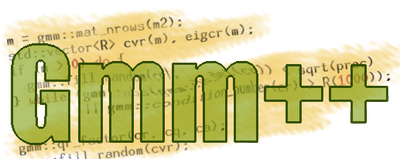
\includegraphics[width=10cm,angle=0]{gmmlogowhitebg}\\[0.2cm]
  a Generic Template Matrix C++ Library \\[0.5cm]
  \fbox{\Huge \sc Short User Documentation} \\[0.5cm]
  { \large Yves {\sc Renard}, Julien {\sc Pommier} \footnote{ \it MIP, INSAT, Complexe scientifique de Rangueil, 31077 Toulouse, France, Yves.Renard@gmm.insa-tlse.fr } } \\[1.0cm]
  \today \\[1.0cm]
}
\htmlonly{
  \xlink{\htmlimg{gmmlogo.png}{the gmm logo}}{http://www-gmm.insa-toulouse.fr/getfem/gmm_intro}\\[2cm]
  a Generic Template Matrix C++ Library \par\par
  {\Huge Short User Documentation } \par
  { \large \xlink{Yves Renard}{mailto:Yves.Renard@gmm.insa-tlse.fr}, \xlink{Julien Pommier}{mailto:Julien.Pommier@gmm.insa-tlse.fr}}\\
  {\it MIP, INSAT, Complexe scientifique de Rangueil, 31077 Toulouse, France.}\par
  \today \par\par
}
\end{center}

% \begin{abstract}
% Basic user documentation for \gmm .
% \end{abstract}


%%%%%%%%%%%%%%%%%%%%%%%%%%%%%%%%%%%%%%%%%%%%%%%%%%%%%%%%%%%%%%%%%%%%%%%%%
%          INTRODUCTION                                                 %
%%%%%%%%%%%%%%%%%%%%%%%%%%%%%%%%%%%%%%%%%%%%%%%%%%%%%%%%%%%%%%%%%%%%%%%%%

\section*{Introduction}

\gmm provides some basic types of sparse and dense matrices and vectors. It provides some generic operations on them (copy, addition, multiplication, sub-vector and sub-matrices, solvers ... ). The syntax of \gmm is very close to MTL and ITL (see http://www.osl.iu.edu/research/mtl/). Especially, the code for most of the iterative solvers has been imported from ITL. The performance of \gmm is also close to the one of MTL, sometimes better. The difference is that basically \gmm has been written to be able to interface other libraries and gives an access to sub matrices and sub vectors in all cases. Also some optimizations has been made for matrix-matrix multiplication, usage of reference has been somewhat cleared, const qualifier usage is clarified, and we hope it is somewhat easier to use.\\ \\[3cm]
\htmlonly{\\\\\\}
Copyright (C) 2000-2020 Yves Renard, Julien Pommier.\\
The program GetFEM is free software; you can redistribute it and/or modify
it under the terms of the GNU Lesser General Public License as published by
the Free Software Foundation; either version 3 of the License, or
(at your option) any later version along with the GCC Runtime Library
Exception either version 3.1 or (at your option) any later version.
This program is distributed in the hope that it will be useful,
but WITHOUT ANY WARRANTY; without even the implied warranty of
MERCHANTABILITY or FITNESS FOR A PARTICULAR PURPOSE.  See the
GNU Lesser General Public License for more details.
You should have received a copy of the GNU  Lesser General Public License
along with this program; if not, write to the Free Software Foundation,
Inc., 51 Franklin Street, Fifth Floor, Boston, MA  02110-1301  USA

\newpage
\tableofcontents
\newpage

\section{How to install and use \gmm}
\index{Install}
Since we use standard GNU tools, the installation of the \gmm library is somewhat standard. Moreover, as \gmm is a template library, no compilation is needed to install it. If the \gmm  archive is on your current directory you can unpack it and enter inside the directory of the distribution  with the commands
\begin{alltt}
  gunzip -c gmm-x.xx.tar.gz | tar xvf -
  cd  gmm-x.xx
\end{alltt}
Then you you have to run the configure script just typing
\begin{alltt}
  ./configure
\end{alltt}
or if you want to set the prefix directory where to install the library you can use the {\tt {-}{-}prefix} option (the default prefix directory is {\tt /usr/local}):
\begin{alltt}
  ./configure --prefix=\textit{dest_dir}
\end{alltt}
then start the installation with
\begin{alltt}
  make install
\end{alltt}
You can also check if your configuration is correct with
\begin{alltt}
  make check
\end{alltt}
which compiles random tests.

If you want to use a different compiler than the one chosen
automatically by the \texttt{./configure} script, just specify its
name on the command line:
\begin{alltt}
  ./configure CXX=mycompiler
\end{alltt}
More specific instructions can be found in the \texttt{README*} files of
the distribution.\\[0.2cm]

Now, to use \gmm in you programs, the simpler manner is to include the file \filename{gmm/gmm.h} which includes all the template library. If the compilation time is too important, the minimum to be included is contained is the file \filename{gmm/gmm\_kernel.h} (vectors and matrix types, blas, sub vector and sub matrices).\\[0.2cm]

DO NOT FORGET to catch errors messages. See the corresponding section.

\section{Matrix and Vector type provided by \gmm}

The convention is that any vector or matrix type (except if it is a  reference)
can be instantiated with the constructors
\begin{cppcode}
  Vector V(n);        // build a vector of size n.
  Matrix M(n, m);     // build a matrix with n rows and m columns.
\end{cppcode}
No other constructor is used inside \gmm and you should not use any other if you want your code
to be compatible with any matrix and vector type.\\[0.2cm]

It is assumed that each vector type interfaced with \gmm allows to
access to a component with the following syntax\\[0.2cm]
\begin{cppcode}
  a = V[i];    // read the ith component of V. \\
  V[i] = b;    // write the ith component of V.
\end{cppcode}$\;$\\[0.2cm]
The write access being available if the vector is not a constant reference. For a matrix\\[0.2cm]
\begin{cppcode}
  a = M(i, j); // read the component at row i and column j of M. \\
  M(i, j) = b; //  write the component at row i and column j of M.
\end{cppcode}$\;$\\[0.2cm]
Again the write access is available if the matrix is not a const reference. Generally, especially for sparse matrices, this access is not very efficient. Linear algebra procedures access to the components of the vectors and matrices via iterators. (see section  \ref{sec:inside}) \\[0.2cm]

It is also not recommended (at all) to use the original copy operator for vectors or matrices. Generally, it will not do the appropriate job. instead, you have to use the method \\[0.2cm]
\begin{cppcode}
  gmm::copy(V, W);  //  W <-- V
\end{cppcode}$\;$\\[0.2cm]
which works for all correctly interfaced matrix and vector type, even if \cpp{V} is not of the same type as \cpp{W} (\cpp{V} could be sparse and \cpp{W} dense for instance). \\[0.2cm]

in \gmm, a vector is not a (n by 1) matrix, it is a one dimensional object. If you need to use a vector as a (n by 1) column matrix or a (1 by n) row matrix, you can do it with
\begin{cppcode}
   gmm::row_vector(V) // gives a reference on V considered as
                      // a (1 by n) row matrix
   gmm::col_vector(V) // gives a reference on V considered as
                      // a (n by 1) col matrix
\end{cppcode}$\;$\\[0.2cm]

In the following, the template parameter \cpp{T} will represent a scalar type like \cpp{double} or \cpp{std::complex<double>}.


\subsection{dense vectors}
\index{std::vector$<$T$>$}
\gmm interfaces \cpp{std::vector<T>} so you can use it as your basic dense vector type.
If you need to interface another type of dense vector you can see in \cpp{gmm/gmm_interface.h}
some examples.
\subsection{sparse vectors}
\index{gmm::wsvector$<$T$>$}
\index{gmm::rsvector$<$T$>$}
\gmm provides two types of sparse vectors: \cpp{gmm::wsvector<T>} and \cpp{gmm::rsvector<T>}. \cpp{gmm::wsvector<T>} is optimized for write operations and \cpp{gmm::rsvector<T>} is optimized for read operations. It should be appropriate to use \cpp{gmm::wsvector<T>} for assembling procedures and then to copy the vector in a \cpp{gmm::rsvector<T>} for the solvers. Those two vector types can be used to create row major or column major matrices (see section \ref{sec:racmat}).

\subsection{skyline vectors}
\index{gmm::slvector$<$T$>$}
The type \cpp{gmm::slvector<T>} defines a skyline vector, in the sense that only an interval of this vector is stored. With this type of vector you can build skyline matrices as \cpp{gmm::row_matrix< gmm::slvector<T> >} (see next section \label{sec:racmat}).

\subsection{generic row and column matrices} \label{sec:racmat}
\index{gmm::row_matrix$<$VECT$>$}
\index{gmm::col_matrix$<$VECT$>$}
\gmm provides the two following types of matrices: \cpp{gmm::row_matrix<VECT>} and \cpp{gmm::col_matrix<VECT>} where \cpp{VECT} should be a valid (i.e. interfaced) vector type.
Those two type of matrices store an array of \cpp{VECT} so the memory is not contiguous. Initializations are
\begin{cppcode}
  gmm::row_matrix< std::vector<double> > M1(10, 10);  // dense row matrix
  gmm::col_matrix< gmm::wsvector<double> > M2(5, 20); // sparse column matrix
\end{cppcode}
Of course \cpp{gmm::row_matrix<VECT>} is a row matrix and it is impossible to access to a particular column of this matrix. 
\index{gmm::mat_nrows(M)}
\index{gmm::mat_ncols(M)}\\

\cpp{gmm::mat_nrows(M)} gives the number of rows of a matrix and \cpp{gmm::mat_ncols(M)} the number of columns.

\subsection{dense matrices}
\index{gmm::dense_matrix$<$T$>$}
A matrix type like \cpp{gmm::row_matrix< std::vector<double> >} or \cpp{gmm::col_matrix< std::vector<double> >} represents a dense matrix. \gmm provides also the type \\[0.2cm]
 \cpp{gmm::dense_matrix<T>}  \\[0.2cm]
which is a dense matrix with a contiguous memory and Fortran type access (column major). It is considered as a column and row matrix (column preferred) which means that you can access both to the columns and rows. This type can be interfaced with Lapack.

\subsection{sparse matrices}
\index{gmm::csr_matrix$<$T$>$}
\index{gmm::csc_matrix$<$T$>$}
Similarly, \cpp{gmm::row_matrix< gmm::wsvector<double> >} or \cpp{gmm::col_matrix< gmm::rsvector<double> >} represents some sparse matrices, but \gmm provides also two types of classical sparse matrix types:  \\[0.2cm]
 \cpp{gmm::csr_matrix<T>} \\
 \cpp{gmm::csc_matrix<T>} \\[0.2cm]
The type \cpp{gmm::csr_matrix<T>} represents a compressed sparse row matrix and \cpp{gmm::csc_matrix<T>} a compressed sparse column matrix. The particularity of these two types of matrices is to be read only, in the sense that it is not possible to access at a particular component to write on it (the operation is too expansive). The only write operation permitted is \cpp{gmm::copy}. The right way to use these matrices is first to execute the write operations on another type of matrix like \cpp{gmm::row_matrix< gmm::wsvector<double> >} then to do a copy:
\begin{cppcode}
  gmm::row_matrix< gmm::wsvector<double> > M1;
  ...
  assembly operation on M1
  ...
  M1(i,j) = b;
  ...
  gmm::csc_matrix<double> M2;
  gmm::clean(M1, 1E-12);
  gmm::copy(M1, M2);
\end{cppcode}
Matrices \cpp{gmm::csr_matrix<T>} and \cpp{gmm::csc_matrix<T>} have the advantage to have a standard format (interfacable with Fortran code) and to have a compact format (contiguous in memory). To be able to be compatible with Fortran programs a second template parameter exists on these type, you can declare
\begin{cppcode}
  gmm::csc_matrix<double, 1> M1;
  gmm::csr_matrix<double, 1> M2;
\end{cppcode}
The ``1'' means that a shift will be done on all the indices.

\section{Input and output with Harwell-Boeing and Matrix Market formats}
\index{Harwell-Boeing format}
\index{Matrix Market format}
Including the file \cpp{gmm/gmm_inoutput.h} you will be able to load and save matrices with Harwell-Boeing and Matrix Market formats. Concerning the Harwell-Boeing format, only the type \cpp{gmm::csc_matrix<double>} and \cpp{gmm::csc_matrix<std::complex<double> >} has been interfaced, so you can execute
\begin{cppcode}
Harwell_Boeing_save("filename", A) // save the csc_matrix A .
Harwell_Boeing_load("filename", A) // load the csc_matrix A.
\end{cppcode}
Of course if you need to save another kind of matrix, you can do first a copy in a \cpp{gmm::csc_matrix}.

Concerning the Matrix Market format, it is possible to save a \cpp{gmm::csc_matrix<double>} or a  \cpp{gmm::csc_matrix<std::complex<double> >} and to load a \cpp{gmm::row_matrix<VECT>} or a \cpp{gmm::col_matrix<VECT>}.
\begin{cppcode}
MatrixMarket_save("filename", A) // save a csc_matrix.
MatrixMarket_load("filename", A) // load a row_matrix or a col_matrix
\end{cppcode}


\section{sub-vectors and sub-matrices}
\index{gmm::sub_interval(first, length)}
It is possible to obtain any sub-vector or sub-matrix of a fully interfaced object. There are four types of sub indexes.
\begin{cppcode}
  gmm::sub_interval(first, length);
\end{cppcode}
represents an interval whose first index is \cpp{first} and length is \cpp{length} ( for instance \cpp{gmm::sub_interval(10, 3);} represents the indexes \cpp{\{10, 11, 12\} }).
\index{gmm::sub_slice(first, length, step)}
\begin{cppcode}
  gmm::sub_slice(first, length, step);
\end{cppcode}
represents also an interval in which one index over \cpp{step} is taken. ( for instance \cpp{gmm::sub_slice(10, 3, 2);} represents the indexes \cpp{\{10, 12, 14\} })
\begin{cppcode}
  gmm::sub_index(CONT c);
\end{cppcode}
represents the sub-index which is the collection of index contained in the container \cpp{c}. For instance
\index{gmm::sub_index(c)}
\begin{cppcode}
  std::vector<size_t> c(3);
  c[0] = 1; c[1] = 3; c[2] = 16;
  gmm::sub_index(c);
\end{cppcode}

represents the indexes \cpp{\{1, 3, 16\} }.\\
{\bf VERY IMPORTANT} : the container \cpp{c} has to be {\bf sorted} from the smaller index to the greater one (i.e. with increasing order) and no repetition is allowed.\\
For unsorted index such as permutation, a special type of sub index is defined:\\

\index{gmm::nsorted_sub_index(c)}
\begin{cppcode}
  gmm::unsorted_sub_index(CONT c);
\end{cppcode}
Some algorithms are a little bit slower with unsorted sub indexes.

\index{gmm::sub_vector(V, subi)}
Now \cpp{gmm::sub_vector(V, subi)} gives a reference to a sub-vector:
\begin{cppcode}
  gmm::vsvector<double> V(10);
  V[5] = 3.0;
  std::cout << gmm::sub_vector(V, gmm::sub_interval(2, 3)) << std::endl;  
\end{cppcode}
prints to the standard output \cpp{V[2], V[3]} and \cpp{V[4]}.\\

\index{gmm::sub_matrix(V, subi1, subi2)}
\cpp{gmm::sub_matrix(V, subi1, subi2)} gives a reference to a sub-matrix. For instance:
\begin{cppcode}
  gmm::col_matrix< gmm::wsvector<double> > M(5, 20);
  M(3, 2) = 5.0;
  std::cout << gmm::sub_matrix(M, gmm::sub_interval(2, 3), gmm::sub_interval(2, 3))
            << std::endl;  
\end{cppcode}
prints to the output a sub-matrix. If the two sub-indexes are equal, it is possible to omit the second. For instance:
\begin{cppcode}
  gmm::col_matrix< gmm::wsvector<double> > M(5, 20);
  M(3, 2) = 5.0;
  std::cout << gmm::sub_matrix(V, gmm::sub_interval(2, 3)) << std::endl;  
\end{cppcode}
The reference on sub_matrix is writable if the corresponding matrix is writable (so you can copy on a sub_matrix, add sub-matrices ...).

\subsection{row and column of a matrix}
\index{gmm::mat_row(M, i)}
\index{gmm::mat_col(M, i)}
\index{gmm::mat_const_row(M, i)}
\index{gmm::mat_const_col(M, i)}
\cpp{gmm::mat_row(M, i)} gives a (possibly writable) reference to the row \cpp{i} of matrix \cpp{M}, and \cpp{gmm::mat_col(M, i)}  gives a (possibly writable) reference to the column \cpp{i}. It is not possible to access to the rows if \cpp{M} is a column matrix and to the columns if it is a row matrix. It is possible to use \cpp{gmm::mat_const_row(M, i)} and \cpp{gmm::mat_const_col(M, i)} to have constant references.

\section{miscellaneous methods}
\index{gmm::vect_size(V)}
\begin{cppcode}
  gmm::vect_size(V); // gives the size of the vector V.
\end{cppcode}

\index{gmm::resize(V, n)}
\index{gmm::resize(M, m, n)}
\index{gmm::reshape(M, m, n)}
\begin{cppcode}
  gmm::resize(V, n); // Change the size of the vector V.
                     // Preserve the min(n, vect_size(V)) first components.
                     // Do not work for references.
  gmm::resize(M, m, n); // Change the dimensions of matrix M.
                        // Preserve the
                        // min(m, mat_nrows(M)) x min(n, mat_ncols(M))
                        // first components. Do not work for references.
  gmm::reshape(M, m, n);  // returns the m-by-n matrix whose elements
                          // are taken columnwise from M.
                          // An error results if M does not have m*m
                          // elements. Works only with dense_matrix<T> for
                          // the moment.
\end{cppcode}

\index{gmm::nnz(V)}
\begin{cppcode}
  gmm::nnz(V); // gives the number of stored components of the vector V.
  gmm::nnz(M); // gives the total number of stored components of the matrix M.
\end{cppcode}



\index{gmm::mat_nrows(M)}
\index{gmm::mat_ncols(M)}
\begin{cppcode}
  gmm::mat_nrows(M) // gives the number of rows of a matrix M.
  gmm::mat_ncols(M) // gives the number of columns of a matrix M.
\end{cppcode}

\index{gmm::write}
\begin{cppcode}
  gmm::write(o, V); // print the vector V to the output stream o.
  gmm::write(o, M); // print the matrix M to the output stream o.
\end{cppcode}
Most of the time it is more convenient to use
\begin{cppcode}
  std::cout << V << std::endl;
  std::cout << M << std::endl;
\end{cppcode}

\index{gmm::clear}
\begin{cppcode}
  gmm::clear(V); // set to zero all the components of the vector V;
  gmm::clear(M); // set to zero all the components of the matrix M;
\end{cppcode}

\index{gmm::clean}
\begin{cppcode}
  gmm::clean(V, 1E-10); // set to zero all the components of the vector V
                        // whose modulus is less or equal to 1E-10
  gmm::clean(M, 1E-10); // idem for a matrix M.
\end{cppcode}

\index{gmm::fill_random}
\begin{cppcode}
  gmm::fill_random(V); // fill a dense vector V with random number
                       //  between 0 and 1
  gmm::fill_random(V, cfill); // fill a dense or sparse vector with random
                       // numbers. cfill should be between 0.0 qnd 1.0 and
                       // represent the ratio of filled components.
  gmm::fill_random(M); // fill a dense matrix M with random number
  gmm::fill_random(M, cfill); // fill a dense or sparse matrix M with random
                       // numbers.
\end{cppcode}

\section{Basic linear algebra operations}
The same choice has been made as in MTL to provide basic operations as functions not as operators. The advantages are that it is clearer to see where are the linear algebra operations in the program and the programming of optimized basic linear operations is greatly simplified.


\subsection{scale and scaled}
\index{gmm::scale}
\index{gmm::scaled}
\cpp{gmm::scale} is used to multiply a vector or a matrix with a scalar factor.
\begin{cppcode}
  gmm::scale(V, 10.0);  // V * 10.0 ---> V
\end{cppcode}
If one not needs to multiply the vector but wants to use the multiplied vector in an expression  \cpp{gmm::scaled } gives a reference to a multiplied vector. This is only a reference, no operation is made until this reference is used somewhere. For instance
\begin{cppcode}
  std::cout << gmm::scaled(V, 10.0) << std::endl;
\end{cppcode}
print to the standard output the vector \cpp{V} multiplied by \cpp{10.0} without changing \cpp{V}.

\subsection{transposition}
\index{gmm::transposed}
\cpp{gmm::transposed(M) } gives a possibily modifiable reference on the transposed matrix of \cpp{M}.

\subsection{imaginary and real part}
\index{gmm::real_part}
\index{gmm::imag_part}
For a complex matrix \cpp{M} or a complex vector \cpp{V}, 
\cpp{gmm::real_part(M)}, \cpp{gmm::real_part(V)}, \cpp{gmm::imag_part(M)} or \cpp{gmm::imag_part(V)} give a possibily modifiable reference on the real or imaginary part of the matrix or vector (for instance \cpp{gmm::clear(gmm::imag_part(M))} will set to zero the imaginary part of a matrix \cpp{M}). These functions cannot be applied to real matrices or vectors.

\subsection{conjugate}
\index{gmm::conjugated}

For a matrix \cpp{M} or a vector \cpp{V}, 
\cpp{gmm::conjugated(M) } and \cpp{gmm::conjugated(V)} give a constant reference on the conjugated vector or matrix. Of course, for a real vectors this has no effect (and no cost at all). Note : \cpp{gmm::conjugated(M) } transposes the matrix \cpp{M} so that this is the hermitian conjugate of $M$. If you need only the conjugate of each component you have to use both transposition and conjugate with \cpp{gmm::conjugated(gmm::transposed(M))} or equivalently  \cpp{gmm::transposed(gmm::conjugated(M))}.


\subsection{add}
\index{gmm::add}
addition of vectors or matrices. It is alway possible to mix different type of vector or matrices in the operations. The following operations are valid:
\begin{cppcode}
  std::vector<double> V1(10);
  gmm::wsvector<double> V2(10);
  gmm::clear(V1);
  ...
  gmm::add(V1, V2); // V1 + V2 --> V2
  cout << V2;

  gmm::add(V1, gmm::scaled(V2, -2.0), V2); // V1 - 2.0 * V2 --> V2
  cout << V2;

  gmm::row_matrix< std::vector<double> > M1(10, 10);
  gmm::col_matrix< gmm::wsvector<double> > M2(1000, 1000);

  // M1 + (sub matrix of M2) ---> (sub matrix of M2)
  gmm::add(M1, gmm::sub_matrix(M2, gmm::sub_interval(4,10)));
\end{cppcode}

IMPORTANT : all the vectors have to have the same size, no resize will be automatically done. If a vector has not the good size, an error will be thrown.

\subsection{mult}
\index{gmm::mult} \index{gmm::mult_add}
Matrix-vector or matrix-matrix multiplication. Again, all the matrices and vectors have to have the good size. The following operations are valid:
\begin{cppcode}
  std::vector<double> V1(10);
  gmm::wsvector<double> V2(10);
  ...
  gmm::row_matrix< std::vector<double> > M1(10, 10);
  ...

  gmm::mult(M1, V2, V1);  // M1 * V2 --> V1

  gmm::mult(M1, V2, V2, V1);  // M1 * V2 + V2 --> V1

  gmm::mult_add(M1, V2, V1);  // M1 * V2 + V1 --> V1

  gmm::mult(M1, gmm::scaled(V2, -1.0), V2, V1);  // M1 * (-V2) + V2 --> V1

  gmm::col_matrix< gmm::wsvector<double> > M2(10, 10);
  gmm::col_matrix< gmm::vsvector<double> > M3(10, 10);
  ...
  
  gmm::mult(M1, M2, M3); // M1 * M2 ---> M3
  
  gmm::mult(gmm::sub_matrix(M1, sub_interval(0, 3)),
            gmm::sub_matrix(M2, sub_interval(4, 3)),
            gmm::sub_matrix(M3, sub_interval(2, 3)));

\end{cppcode}

\subsection{norms}
\index{gmm::vect_norm1(V)}
\index{gmm::vect_norm2(V)}
\index{gmm::vect_dist2(V1, V2)}
\index{gmm::vect_inf(V)}
\index{gmm::mat_norm2(M)}
\index{gmm::mat_normmax(M)}

\begin{cppcode}
  gmm::vect_norm1(V)  // sum of the modulus of the components of vector V.\\
  gmm::vect_norm2(V)  // Euclidean norm of vector V.
  gmm::vect_dist2(V1, V2)  // Euclidean distance between V1 and V2.
  gmm::vect_inf(V)    // infinity norm of vector V.
  gmm::mat_euclidean_norm(M) // Euclidean norm of matrix \cpp{M}
                             // (called also Fr\"obenius norm).
  gmm::mat_normmax(M) // Max norm (defined as max(|m_ij|; i,j ))
  gmm::mat_norm1(M)   // max(sum(|m_ij|, i), j)
  gmm::mat_norminf(M) // max(sum(|m_ij|, j), i)

\end{cppcode}
\subsection{trace}
\index{gmm::mat_trace(M)}
\cpp{gmm::mat_trace(M)} gives the trace of matrix \cpp{M}.

\subsection{scalar product} 
\index{gmm::vect_sp(V1, V2)}
\index{gmm::vect_hp(V1, V2)}

  for vectors only, \cpp{gmm::vect_sp(V1, V2)} gives the scalar product between \cpp{V1} and \cpp{V2}. For complex vectors, this do not conjugate \cpp{V1}, you can use \cpp{gmm::vect_sp(V1, gmm::conjugated(V2))} or \cpp{gmm::vect_hp(V1, V2) } which is equivalent.

\section{Solving triangular systems}

If \cpp{M} is a triangular matrix (upper or lower) and \cpp{X} a vector containing the right hand side, the following procedures solve the system $x \leftarrow M^{-1}x$. The vector \cpp{X} contains the result.
\begin{cppcode}
   gmm::upper_tri_solve(M, X, false) // Solving an upper triangular system
   gmm::upper_tri_solve(M, X, true)  // Solving an upper triangular system
                                     // assuming there is 1 on the diagonal
   gmm::lower_tri_solve(M, X, false) // Solving a lower triangular system
   gmm::lower_tri_solve(M, X, true)  // Solving a lower triangular system
                                     // assuming there is 1 on the diagonal
\end{cppcode}
components which are lower the diagonal are ignored by \cpp{gmm::upper_tri_solve} and components which are upper the diagonal are ignored by \cpp{gmm::lower_tri_solve}.

\section{Dense LU decomposition}

The following procedures are available in the file \filename{gmm/gmm\_dense\_lu.h} for dense real and complex matrices (\cpp{gmm::dense_matrix<T>}, \cpp{gmm::row_matrix< std::vector<T> >} and \cpp{gmm::col_matrix< std::vector<T> >})

\begin{cppcode}
gmm::lu_factor(M, ipvt) : compute the LU factorization of M in M. ipvt should be
                     an std::vector<size_t> (of size gmm::mat_nrows(M))
                     which will contain the indices of the pivots.

gmm::lu_solve(LU, ipvt, x, b) : solve the system LUx = b. LU is the LU
                           factorization which has to be computed first.

gmm::lu_solve(M, x, b) : solve the system Mx=b calling the lu factorization on
                    a copy of M.

gmm::lu_solve_transposed(LU, ipvt, x, b) : solve the system transposed(LU)x = b.
                                      LU is the LU factorization which
                                      has to be computed first.

gmm::lu_inverse(LU, ipvt, A) : compute the inverse of LU in A. LU is the LU
                          factorization which has to be computed first

gmm::lu_inverse(A) : invert A calling the LU factorization and the latter
                procedure.

gmm::lu_det(LU, ipvt) : compute the determinant of LU. LU is the LU
                   factorization which has to be computed first

gmm::lu_det(A) : compute the determinant of A calling the LU factorization
            and the latter function.
\end{cppcode}

\section{Dense QR factorisation, eigenvalues and eigenvectors}
The following procedures are available in the file \filename{gmm/gmm\_dense\_qr.h} for dense real and complex matrices.
\index{gmm::qr_factor(M, Q, R)}
\index{gmm::implicit_qr_algorithm(M, eigval, tol)}
\index{gmm::symmetric_qr_algorithm(M, eigval, tol)}

\begin{cppcode}
  gmm::qr_factor(M, Q, R) // compute the QR factorization of M in Q and R
                          // (Householder version)

  implicit_qr_algorithm(M, eigval, double tol = 1E-16) // compute the
     // eigenvalues of M using the implicit QR factorisation (Householder and
     // Francis QR step version). eigval should be a vector of appropriate size
     // in which the eigenvalues will be computed. If the matrix have 
     // complex eigenvalues, please use a complex vector.

  implicit_qr_algorithm(M, eigval, shvect, double tol = 1E-16) // idem, 
     // compute additionally the schur vectors in the matrix shvect.

  symmetric_qr_algorithm(M, eigval, double tol = 1E-16) // idem for symmetric
     // real and hermitian complex matrices (based on Wilkinson QR step)

  symmetric_qr_algorithm(M, eigval, eigvect, double tol = 1E-16) // idem,
     // compute additionally the eigenvectors in the matrix eigvect.

\end{cppcode}

Remark : The computation of eigenvectors for non hermitian matrices is not yet implemented. You can use for the moment the functions \cpp{geev_interface_left} and \cpp{geev_interface_right} from the LAPACK interface (see \cpp{gmm/gmm_lapack_interface.h}. These LAPACK functions compute right and left eigen vectors. 
                   
\section{Condition number estimation}
\index{gmm::condest}
The following function defined in the file \filename{gmm/gmm\_condition\_number.h}
\begin{cppcode}
   condition_number(M)
\end{cppcode}
compute the condition number of a matrix \cpp{M}. For the moment, this function uses a dense QR algorithm and thus is only usable for dense matrices.

\section{Iterative solvers}
Most of the solvers provided in \gmm come form ITL with slight modifications (gmres has been optimized and adapted for complex matrices). Include the file \filename{gmm/gmm_iter_solvers.h} to use them.

\subsection{iterations}
\index{gmm::iteration}
  The iteration object of \gmm is a modification of the one in ITL. This is not a template type as in ITL. 

The simplest initialization is
\begin{cppcode}
  gmm::iteration iter(2.0E-10);
\end{cppcode}
where \cpp{2.0E-10} is the (relative) residual to be obtained to have the convergence.
Some possibilities :
\begin{cppcode}
  iter.set_noisy(n) // n = 0 : no output
                    // n = 1 : output of iterations on the standard output
                    // n = 2 : output of iterations and sub-iterations 
                    //         on the standard output
                    // ...
  iter.get_iteration() // after a computation, gives the number of
                       // iterations made.
  iter.converged()     // true if the method converged.
  iter.set_maxiter(n)  // Set the maximum of iterations.
                       // A solver stops if the maximum of iteration is 
                       // reached, iter.converged() is then false.
\end{cppcode}

\subsection{various solvers}
Here is the list of available linear solvers.
\index{gmm::cg}
\index{gmm::bicgstab}
\index{gmm::gmres}
\index{gmm::qmr}
\index{gmm::constrained_cg}
\begin{cppcode}
  gmm::row_matrix< std::vector<double> > A(10, 10);  // The matrix
  std::vector<double> B(10); // Right hand side
  std::vector<double> X(10); // Unknown
  gmm::identity_matrix PS;   // Optional scalar product for cg
  gmm::identity_matrix PR;   // Optional preconditioner
  ...
  gmm::iteration iter(10E-9);// Iteration object with the max residu
  size_t restart = 50;       // restart parameter for GMRES
  
  gmm::cg(A, X, B, PS, PR, iter); // Conjugate gradient

  gmm::bicgstab(A, X, B, PR, iter); // BICGSTAB BiConjugate Gradient Stabilized

  gmm::gmres(A, X, B, PR, restart, iter) // GMRES generalized minimum residual

  gmm::qmr(A, X, B, PR, iter) // Quasi-Minimal Residual method.

  gmm::least_square_cg(A, X, B, iter) // unpreconditionned least square CG.
\end{cppcode}

The solver \cpp{gmm::constrained_cg(A, C, X, B, PS, PR, iter);} solve a system with linear constaints, \cpp{C} is a matrix which represents the constraints. But it is still experimental.\\

(Version 1.7) The solver \cpp{gmm::bfgs(F, GRAD, X, restart, iter)} is a BFGS quasi-Newton algorithm with a Wolfe line search for large scale problems. It minimizes the function \cpp{F} without constraints, be given its gradient \cpp{GRAD}. \cpp{restart} is the max number of stored update vectors.

\subsection{various preconditioners}
The following preconditioners, to be used with linear solvers, are available: 
\index{gmm::diagonal_precond}
\index{gmm::ilu_precond}
\index{gmm::ilut_precond}
\index{gmm::ilutp_precond}
\index{gmm::mr_approx_inverse_precond}
\begin{cppcode}
  gmm::identity_matrix P;   // No preconditioner 

  gmm::diagonal_precond<matrix_type> P(SM); // diagonal preconditioner
 
  gmm::mr_approx_inverse_precond<matrix_type> P(SM, 10, 10E-17);
                                               // preconditioner based on MR
                                               // iterations

  gmm::ildlt_precond<matrix_type> P(SM); // incomplete (level 0) ldlt 
                                        // preconditioner. Fast to be
                                        // conputed but less efficient than
                                        // gmm::ildltt_precond.

  // incomplete ldlt with k fill-in and threshold preconditioner.
  // Efficient but could be costly.
  gmm::ildltt_precond<matrix_type> P(SM, k, threshold);

  gmm::ilu_precond<matrix_type> P(SM);  // incomplete (level 0) ilu 
                                        // preconditioner. Very fast to be
                                        // computed but less efficient than
                                        // gmm::ilut_precond.


  // incomplete LU with k fill-in and threshold preconditioner.
  // Efficient but could be costly.
  gmm::ilut_precond<matrix_type> P(SM, k, threshold);

  // incomplete LU with k fill-in, threshold and column pivoting preconditioner.
  // Try it when ilut encounter too small pivots. 
  gmm::ilutp_precond<matrix_type> P(SM, k, threshold);
\end{cppcode}

Except \cpp{ildltt\_precond}, all these precontionners come from ITL. \cpp{ilut_precond} has been optimized and simplified and \cpp{cholesky_precond} has been corrected and transformed in an incomplete LDLT preconditionner for stability reasons (similarly, we add \cpp{choleskyt_precond} which is in fact an incomplete LDLT with threshold preconditionner). Of course, \cpp{ildlt\_precond} and \cpp{ildltt_precond} are designed for symmetric real or hermitian complex matrices to be use principaly with cg.

\subsection{Additive Schwarz method}
The additive Schwarz method is a decomposition domain method allowing the resolution of huge linear systems (see \cite{SCHADD} for the principle of the method).

For the moment, the method is not parallelized (this should be done soon ...). The call is the following: 

\begin{cppcode}
 gmm::sequential_additive_schwarz(A, u, f, P, vB, iter, local_solver, global_solver)
\end{cppcode}                           
\cpp{A} is the matrix of the linear system. \cpp{u} is the unknown vector. \cpp{f} is the right hand side. \cpp{P} is an eventual preconditioner for the local solver. \cpp{vB} is a vector of rectangular sparse matrices (\cpp{of type const std::vector<vBMatrix>}, where \cpp{vBMatrix} is a sparse matrix type), each of these matrices is of size $N \times N_i $ where $N$ is the size of \cpp{A} and $N_i$ the number of variables in the $i^{th}$ sub-domain ; each column of the matrix is a base vector of the sub-space representing the $i^{th}$ sub-domain. \cpp{iter} is an iteration object. \cpp{local_solver} has to be chosen in the list \cpp{gmm::using_gmres(), gmm::using_bicgstab(), gmm::using_cg(), gmm::using_qmr()} and  \cpp{gmm::using_superlu()} if SuperLu is installed. \cpp{global_solver} has to be chosen in the list \cpp{gmm::using_gmres(), gmm::using_bicgstab(), gmm::using_cg(), gmm::using_qmr()}.\\

The test program \cpp{schwarz_additive.C} is the directory \cpp{tests} of Getfem++ is an example of the resolution with the additive Schwarz method of an elastostatic problem with the use of coarse mesh to make a better preconditioning (i.e. one of the sub-domains represents in fact a coarser mesh).\\

In the case of multiple solves with the same linear system, it is possible to store the preconditioners or the LU factorisations to save computation time.\\

A (too) simple program in \cpp{gmm/gmm_domain_decomp.h} allows to build a regular domain decomposition with a certain ratio of overlap. It directly produces the vector of matrices \cpp{vB} for the additive Schwarz method.

\section{Catch errors}
\index{errors}

Errors used in \gmm are defined in the file \filename{gmm/gmm\_except.h}. In order to make easier  the error catching all errors derive from the type \cpp{std::logic\_error} defined in the file \cpp{ stdexcept} of the S.T.L.\\[0.5cm]
A standard procedure, \cpp{GMM\_STANDARD\_CATCH\_ERROR}, is defined in \cpp{gmm/gmm\_except.h}. This procedure catches all errors and print the error message when an error occurs. It can be used in the main procedure of the program as follows\\[0.5cm]
\begin{cppcode}
  int main(void) \{ 
    try \{ 
      ... main program ... 
        \} 
     GMM\_STANDARD\_CATCH\_ERROR;
  \}
\end{cppcode}

It is highly recommended to catch the errors at least in the main function, because if you do not so, you will not be able to see error messages.

\section{Interface with BLAS, LAPACK or ATLAS}
\index{LAPACK} \index{ATLAS}

For better performance on dense matrices, it is possible to interface some operations of the type \cpp{gmm::dense_matrix<T>} with \cpp{LAPACK} (http://www.netlib.org/lapack/) or \cpp{ATLAS} (http://math-atlas.sourceforge.net/), for \cpp{T = float, double, std::complex<float> or std::complex<double>}. In fact, concerning \cpp{ATLAS} no specific interface has been made untill now, so the fortran interface of \cpp{ATLAS} should be used.

to use this interface you have first to define \cpp{GMM_USES_LAPACK} before including \gmm \ files :

\begin{cppcode}
  \#define GMM_USES_LAPACK
  \#include <gmm/gmm.h>

  ... your code
\end{cppcode}

or specify -DGMM_USES_LAPACK on the command line of your compiler. Of course, you have also to link \cpp{LAPACK} or \cpp{ATLAS} libraries. For example on a standard linux configuration and g++ compiler the adding libraries to link \cpp{LAPACK} are
\begin{cppcode}
  g++ ...  -llapack -lblas -lg2c
\end{cppcode}
and to link  \cpp{ATLAS}
\begin{cppcode}
  g++ ... /usr/lib/atlas/liblapack.a /usr/lib/atlas/libblas.a -latlas -lg2c
\end{cppcode}

Ask your system administrator if this configuration does not work.

The following operations are interfaced:
\begin{cppcode}
  vect_norm2(std::vector<T>)                                           
                                                                        
  vect_sp(std::vector<T>, std::vector<T>)                               
  vect_sp(scaled(std::vector<T>), std::vector<T>)                       
  vect_sp(std::vector<T>, scaled(std::vector<T>))                       
  vect_sp(scaled(std::vector<T>), scaled(std::vector<T>))               
                                                                        
  vect_hp(std::vector<T>, std::vector<T>)                               
  vect_hp(scaled(std::vector<T>), std::vector<T>)                       
  vect_hp(std::vector<T>, scaled(std::vector<T>))                       
  vect_hp(scaled(std::vector<T>), scaled(std::vector<T>))               
                                                                        
  add(std::vector<T>, std::vector<T>)                                   
  add(scaled(std::vector<T>, a), std::vector<T>)                         

  mult(dense_matrix<T>, dense_matrix<T>, dense_matrix<T>)               
  mult(transposed(dense_matrix<T>), dense_matrix<T>, dense_matrix<T>)   
  mult(dense_matrix<T>, transposed(dense_matrix<T>), dense_matrix<T>)   
  mult(transposed(dense_matrix<T>), transposed(dense_matrix<T>),        
       dense_matrix<T>)                                                 
  mult(conjugated(dense_matrix<T>), dense_matrix<T>, dense_matrix<T>)   
  mult(dense_matrix<T>, conjugated(dense_matrix<T>), dense_matrix<T>)   
  mult(conjugated(dense_matrix<T>), conjugated(dense_matrix<T>),        
       dense_matrix<T>)                                                 
                                                                        
  mult(dense_matrix<T>, std::vector<T>, std::vector<T>)                 
  mult(transposed(dense_matrix<T>), std::vector<T>, std::vector<T>)     
  mult(conjugated(dense_matrix<T>), std::vector<T>, std::vector<T>)     
  mult(dense_matrix<T>, scaled(std::vector<T>), std::vector<T>)         
  mult(transposed(dense_matrix<T>), scaled(std::vector<T>),             
       std::vector<T>)                                                  
  mult(conjugated(dense_matrix<T>), scaled(std::vector<T>),             
       std::vector<T>)

  mult_add(dense_matrix<T>, std::vector<T>, std::vector<T>)             
  mult_add(transposed(dense_matrix<T>), std::vector<T>, std::vector<T>) 
  mult_add(conjugated(dense_matrix<T>), std::vector<T>, std::vector<T>) 
  mult_add(dense_matrix<T>, scaled(std::vector<T>), std::vector<T>)     
  mult_add(transposed(dense_matrix<T>), scaled(std::vector<T>),         
           std::vector<T>)                                              
  mult_add(conjugated(dense_matrix<T>), scaled(std::vector<T>),         
           std::vector<T>)                                              
                                                                        
  mult(dense_matrix<T>, std::vector<T>, std::vector<T>, std::vector<T>) 
  mult(transposed(dense_matrix<T>), std::vector<T>, std::vector<T>,     
       std::vector<T>)                                                  
  mult(conjugated(dense_matrix<T>), std::vector<T>, std::vector<T>,     
       std::vector<T>)                                                  
  mult(dense_matrix<T>, scaled(std::vector<T>), std::vector<T>,         
       std::vector<T>)                                                  
  mult(transposed(dense_matrix<T>), scaled(std::vector<T>),             
       std::vector<T>, std::vector<T>)                                  
  mult(conjugated(dense_matrix<T>), scaled(std::vector<T>),             
       std::vector<T>, std::vector<T>)                                  
  mult(dense_matrix<T>, std::vector<T>, scaled(std::vector<T>),         
       std::vector<T>)                                                  
  mult(transposed(dense_matrix<T>), std::vector<T>,                     
       scaled(std::vector<T>), std::vector<T>)                          
  mult(conjugated(dense_matrix<T>), std::vector<T>,                     
       scaled(std::vector<T>), std::vector<T>)                          
  mult(dense_matrix<T>, scaled(std::vector<T>), scaled(std::vector<T>), 
    std::vector<T>)                                                     
  mult(transposed(dense_matrix<T>), scaled(std::vector<T>),             
       scaled(std::vector<T>), std::vector<T>)                          
  mult(conjugated(dense_matrix<T>), scaled(std::vector<T>),             
       scaled(std::vector<T>), std::vector<T>)                          
                                                                        
  lower_tri_solve(dense_matrix<T>, std::vector<T>, k, b)                
  upper_tri_solve(dense_matrix<T>, std::vector<T>, k, b)                
  lower_tri_solve(transposed(dense_matrix<T>), std::vector<T>, k, b)    
  upper_tri_solve(transposed(dense_matrix<T>), std::vector<T>, k, b)    
  lower_tri_solve(conjugated(dense_matrix<T>), std::vector<T>, k, b)    
  upper_tri_solve(conjugated(dense_matrix<T>), std::vector<T>, k, b)    
                                                                        
  lu_factor(dense_matrix<T>, std::vector<int>)                          
  lu_solve(dense_matrix<T>, std::vector<T>, std::vector<T>)             
  lu_solve(dense_matrix<T>, std::vector<int>, std::vector<T>,           
           std::vector<T>)                                              
  lu_solve_transposed(dense_matrix<T>, std::vector<int>, std::vector<T>,
           std::vector<T>)                                              
  lu_inverse(dense_matrix<T>)                                           
  lu_inverse(dense_matrix<T>, std::vector<int>, dense_matrix<T>)        
                                                                        
  qr_factor(dense_matrix<T>, dense_matrix<T>, dense_matrix<T>) 

  implicit_qr_algorithm(dense_matrix<T>, std::vector<T>)
  implicit_qr_algorithm(dense_matrix<T>, std::vector<T>,
                        dense_matrix<T>)                               
  implicit_qr_algorithm(dense_matrix<T>, std::vector<std::complex<T> >)
  implicit_qr_algorithm(dense_matrix<T>, std::vector<std::complex<T> >,
                        dense_matrix<T>)                               
\end{cppcode}

Of course, it is not difficult to interface another operation if needed.

\section{Interface with SuperLU}

It is possible to call SuperLU 3.0 (http://crd.lbl.gov/\verb\~\xiaoye/SuperLU/) from \gmm. The following function defined in the file \filename{gmm/gmm_superlu_interface.h} is available

\begin{cppcode}
  SuperLU_solve(A, X, B, condest, permc_spec = 1)
\end{cppcode}
solves the system \cpp{AX = B} where A is a sparse matrix of base type \cpp{float, double, std::complex<float>, or std::complex<double>}. \cpp{permc_spec} should be 0, 1 or 2 for respectively use the natural ordering, use minimum degree ordering on structure of \cpp{A'A} or use minimum degree ordering on structure of \cpp{A'+A} (1 is the default value), \cpp{condest} should be a reference on a double, it returns an estimate of the condition number of the matrix \cpp{A}.\\

To use these functions, you need to install SuperLU and compile your code with the additional options:
\begin{cppcode}
g++ ...  -DGMM_USES_SUPERLU (dir_of_superlu)/superlu.a -lblas -I(dir_of_superlu)
\end{cppcode}


Some other functionalities of SuperLU can be interfaced. \\


\section{How to use \gmm with QD type (double-double and quad-double)}

The QD library (see http://www.cs.berkeley.edu/\verb\~\yozo or http://www.nersc.gov/\verb\~\dhb/mpdist/mpdist.html) is an efficient library for double-double (32 decimal digits) and quad-double (approx. 64 decimal digits). Once you installed this library on your system you have to link your program with QD library (with -lqd). In your program, include the header files of QD with
\begin{cppcode}
#include <qd/dd.h>
#include <qd/qd.h>
#include <qd/fpu.h>
\end{cppcode}

Then the two type \cpp{dd_real} and \cpp{qd_real} will be usable with \gmm. You will also be able to use \cpp{std::complex<dd_real>} and \cpp{std::complex<qdreal>}\\

IMPORTANT : do not forget to initialize QD before using it with the following call
\begin{cppcode}
unsigned int old_cw;
fpu_fix_start(&old_cw);
\end{cppcode}
This disables the 80 bits precision of x86 processors which conflicts with QD. Once you finished to use QD you can reactivate it with
\begin{cppcode}
fpu_fix_end(&old_cw);
\end{cppcode}
(see the QD documentation for more details).


\section{First steps with \gmm} \label{sec:inside}

\subsection{How can I invert a matrix ?}
It is not possible in \gmm to invert all kind of matrices. For the moment, the only mean to invert a matrix is to use the dense LU decomposition (thus, only for dense matrices). An example
\begin{cppcode}
  gmm::dense_matrix<double> M(3, 3), M2(3,3), M3(3,3);
  gmm::copy(gmm::identity_matrix(), M);  // M = Id.
  gmm::scale(M, 2.0);                    // M = 2 * Id.
  M(1,2) = 1.0;

  gmm::copy(M, M2);  
 
  gmm::lu_inverse(M);

  gmm::mult(M, M2, M3);

  std::cout << M << " times " << M2 << " is equal to " << M3 << endl;
\end{cppcode}
see the section corresponding to dense LU decomposition for more details. The type \cpp{gmm::dense_matrix<double>} can be replaced by \cpp{gmm::row_matrix< std::vector<double> >} or \cpp{gmm::col_matrix< std::vector<double> >}.

\subsection{How can I solve a linear system ?}
You have more than one possibility to solve a linear system. If you have a dense matrix, the best may be to use the LU decomposition. An example
\begin{cppcode}
  gmm::dense_matrix<double> M(3, 3);
  gmm::clear(M);                  // M = 0.
  M(0,0) = M(1,1) = M(2,2) = 2.0; // M = 2 * Id.
  M(1,2) = 1.0;

  std::vector<double> X(3), B(3), Bagain;
  B[0] = 1.0; B[1] = 2.0; B[2] = 3.0;  // B = [1 2 3]
 
  gmm::lu_solve(M, X, B);

  gmm::mult(M, X, Bagain);

  std::cout << M << " times " << X << " is equal to " << Bagain << endl;
\end{cppcode}

If, now, you have a sparse system coming for example from a pde discretization, you have various iterative solvers, with or without preconditioners. This is an example with a precontionned GMRES:
 \begin{cppcode}
  int nbdof = 1000; // number of degrees of freedom.
  gmm::row_matrix< gmm::rsvector<double> > M(nbdof, nbdof); // a sparse matrix
  std::vector<double> X(nbdof), B(nbdof); // Unknown and left hand side.

  ... here the assembly of the pde discretization stiffness matrix ...
  ... and left hand side ...


  // computation of a preconditioner (ILUT)
  gmm::ilut_precond< gmm::row_matrix< gmm::rsvector<double> > > P(M, 10, 1e-4);

  gmm::iteration iter(1E-8);  // defines an iteration object, with a max residu of 1E-8

  gmm::gmres(M, X, B, P, 50, iter);  // execute the GMRES algorithm

  std::cout << "The result " << X << endl;
\end{cppcode}

\subsection{How can I transform a vector into a matrix and reshape it ?}
In \gmm, a vector is not considered as a matrix. If you need to use a vector as a (1 by n) row matrix or (n by 1) column matrix in a computation, you have to use
\begin{cppcode}
   gmm::row_vector(V) // gives a reference on V considered as
                      // a (1 by n) row matrix
   gmm::col_vector(V) // gives a reference on V considered as
                      // a (n by 1) col matrix
\end{cppcode}
for instance, you can transform a vector into a dense matrix with
\begin{cppcode}
  std::vector<double> V(50);

  // ... computation of V

  gmm::dense_matrix<double> M(1, gmm::vect_size(V));
  gmm::copy(gmm::row_vector(V), M);
\end{cppcode}

Then you can also reshape matrix \cpp{M} with
\begin{cppcode}
  gmm::reshape(M, 10, 5);
\end{cppcode}

\subsection{What is the better way to resize a matrix ?}
You can change the dimensions of a matrix, if it is not a reference, using
\begin{cppcode}
  gmm::resize(M, m, n);
\end{cppcode}
This function respects the intersection between the original matrix and the resized matrix, and new components are set to zero. An important thing is that it is based on the resize method of \cpp{std::vector}, thus no memory free is done when the size of the new matrix is smaller than the original one.\\[0.5cm]

If you do not need to keep old values of the components, or if you want to really free the surplus of memory, you can resize a matrix using \cpp{std::swap} as follows
\begin{cppcode}
  MATRIX_TYPE M(m1, n1);

  ... your code

  std::swap(M, MATRIX_TYPE(m2, n2)); // resize matrix M.
\end{cppcode}
Of course, this works also for a vector.


\section{Deeper inside \gmm}

\subsection{The linalg_traits structure}
\index{linalg_traits}
The major principle of \gmm is that each vector and matrix type has a corresponding structure (which is never instantiated) named \cpp{linalg_traits} containing all informations on it. For instance, the component \cpp{linalg_type} of this structure is set to \cpp{abstract_vector} or \cpp{abstract_matrix} if the corresponding type represent a vector or a matrix. If \cpp{V} is an interfaced type of vector and \cpp{M} an interface type of matrix, it is possible to access to this component with
\begin{cppcode}
  typename gmm::linalg_traits<V>::linalg_type ...  // should be abstract_vector
  typename gmm::linalg_traits<M>::linalg_type ...  // should be abstract_matrix
\end{cppcode}
The types \cpp{abstract_vector} and \cpp{abstract_matrix} are defined in \cpp{gmm/gmm_def.h}. They are void type allowing to specialize generic algorithms.\\

For a vector type, the following informations are available
\begin{cppcode}
  typename gmm::linalg_traits<V>::value_type     --> type of the components of the
                                                     vector
  typename gmm::linalg_traits<V>::reference      --> type of reference on a component
  typename gmm::linalg_traits<V>::is_reference   --> if the vector is a simple
                                                     reference or an instantiated vector
  typename gmm::linalg_traits<V>::linalg_type    --> should be abstract_vector
  typename gmm::linalg_traits<V>::index_sorted    --> linalg_true or linalg_false
  typename gmm::linalg_traits<V>::const_iterator --> const iterator to iterate on the
                                                     components of the vector in 
                                                     order to read them.
  typename gmm::linalg_traits<V>::iterator       --> iterator to iterate on the
                                                     components of the vector in
                                                     order to read or write them.
  typename gmm::linalg_traits<V>::storage_type   --> should be abstract_sparse,
                                                     abstract_skyline or
                                                     abstract_dense

  typename gmm::linalg_traits<V>::origin_type    --> the type of vector itself
                                                     or the type of referenced
                                                     vector for a reference.
 
  gmm::linalg_traits<V>::size(v)     --> a method which gives the size of the vector.
  gmm::linalg_traits<V>::begin(v)    --> a method which gives an iterator on the
                                         beginning of the vector
  gmm::linalg_traits<V>::end(v)      --> iterator on the end of the vector
  gmm::linalg_traits<V>::origin(v)   --> gives a void pointer allowing to identify
                                         the vector
  gmm::linalg_traits<V>::do_clear(v) --> make a clear on the vector

  gmm::linalg_traits<V>::access(o, it, ite, i) --> return the ith component or a
                                          reference on the ith component. o is a
                                          pointer o type ``origin_type *'' or 
                                          ``const origin_type *''.

  gmm::linalg_traits<V>::clear(o, it, ite) --> clear the vector. o is a
                                          pointer o type ``origin_type *'' or 
                                          ``const origin_type *''.
\end{cppcode}
and for a matrix type 
\begin{cppcode}
  typename gmm::linalg_traits<M>::value_type     --> type of the components of the
                                                     matrix
  typename gmm::linalg_traits<M>::reference      --> type of reference on a component
  typename gmm::linalg_traits<M>::is_reference   --> if the matrix is a simple
                                                     reference or an instantiated matrix
  typename gmm::linalg_traits<M>::linalg_type    --> should be abstract_matrix
  typename gmm::linalg_traits<M>::storage_type   --> should be abstract_sparse,
                                                     abstract_skyline or
                                                     abstract_dense
  typename gmm::linalg_traits<M>::index_sorted    --> linalg_true or linalg_false
  typename gmm::linalg_traits<M>::sub_orientation --> should be row_major, col_major
                                                      row_and_col or col_and_row.
  typename gmm::linalg_traits<M>::sub_col_type      --> type of reference on a column
                                                      (if the matrix is not row_major)
  typename gmm::linalg_traits<M>::const_sub_col_type --> type of const reference on a 
                                                       column
  typename gmm::linalg_traits<M>::col_iterator      --> iterator on the columns
  typename gmm::linalg_traits<M>::const_col_iterator --> const iterator on the columns
  typename gmm::linalg_traits<M>::sub_row_type      --> type of reference on a row
                                                      (if the matrix is not col_major)
  typename gmm::linalg_traits<M>::const_sub_row_type --> type of const reference on a 
                                                       row
  typename gmm::linalg_traits<M>::const_row_iterator --> const iterator on the rows
  typename gmm::linalg_traits<M>::row_iterator       --> iterator on the rows

  typename gmm::linalg_traits<M>::origin_type    --> the type of vector itself
                                                     or the type of referenced
                                                     vector for a reference.

  gmm::linalg_traits<M>::nrows(m)     --> methods which gives the number of rows of
                                          the matrix
  gmm::linalg_traits<M>::ncols(m)     --> number of columns
  gmm::linalg_traits<M>::row_begin(m) --> iterator on the first row (if not col_major)
  gmm::linalg_traits<M>::row_end(m)   --> iterator on the end of the rows
  gmm::linalg_traits<M>::col_begin(m) --> iterator on the first column
                                          (if not row_major)
  gmm::linalg_traits<M>::col_end(m)   --> iterator on the end of the columns
  gmm::linalg_traits<M>::row(it)      --> gives the reference on a row with an iterator
                                          (if not col_major)
  gmm::linalg_traits<M>::col(it)      --> gives the reference on a column with an
                                          iterator  (if not row_major)
  gmm::linalg_traits<M>::origin(m)    --> gives a void pointer allowing to identify
                                          the matrix
  gmm::linalg_traits<M>::access(it,i) --> return the ith component or a reference 
                                          on the ith component of the row or
                                          column pointed by it.
  gmm::linalg_traits<M>::do_clear(m)  --> make a clear on the matrix
\end{cppcode}

This is this structure you have to fill in to interface a new vector or matrix type. You can see some examples in \cpp{gmm/gmm_interface.h} . Most of the generic algorithms are in \cpp{gmm/gmm_blas.h} .


\subsection{How to iterate on the components of a vector}

Here is an example which accumulate the components of a vector. It is assumed that \cpp{V} is a vector type and \cpp{v} an instantiated vector.

\begin{cppcode}
  
  typename gmm::linalg_traits<V>::value_type r(0); // scalar in which we accumulate
  typename gmm::linalg_traits<V>::const_iterator it = vect_const_begin(v); // beginning 
                                                                           // of v
  typename gmm::linalg_traits<V>::const_iterator ite = vect_const_end(v); // end of v

  for (; it != ite; ++it)  // loop on the components
    r += *it;              // accumulate the components

\end{cppcode}

This piece of code will work with every kind of interfaced vector.\\

For sparse or skyline vectors, it is possible to obtain the index of the components pointed by the iterator with \cpp{it.index()}. Here is the example of the scalar product of two sparse or skyline vectors, assuming \cpp{V1} and \cpp{V2} are two vector types and \cpp{v1}, \cpp{v2} two corresponding instantiated vectors.
\begin{cppcode}
   typename gmm::linalg_traits<V1>::const_iterator it1 = vect_const_begin(v1),
   typename gmm::linalg_traits<V1>::const_iterator ite1 = vect_const_end(v1);
   typename gmm::linalg_traits<V2>::const_iterator it2 = vect_const_begin(v2),
   typename gmm::linalg_traits<V2>::const_iterator ite2 = vect_const_end(v2);
   typename gmm::linalg_traits<V1>::value_type r(0); // it is assumed that V2 have a
                                                // compatible value_type

   while (it1 != ite1 && it2 != ite2) \{  // loops on the components
     if (it1.index() == it2.index()) \{
       res += (*it1) * (*it2));          // if the indexes are equals accumulate
       ++it1;
       ++it2;
     \}
     else if (it1.index() < it2.index())
       ++it1;
     else
       ++it2;
   \}
\end{cppcode}
This algorithm use the fact that indexes are increasing in a sparse vector. This code will not work for dense vectors because dense vector iterators do not have the method \cpp{it.index()}.

\subsection{How to iterate on a matrix}

You can iterate on the rows of a matrix if it is not a column major matrix and on the columns of a matrix if it is not a row major matrix (the type \cpp{gmm::dense_matrix<T>} has is sub orientation type as col_and_rox, so you can iterate on both rows and columns).

If you need not to be optimal, you can use a basic loop like that
\begin{cppcode}
  for (size_t i = 0; i < gmm::mat_nrows(m); ++i) \{
    typename gmm::linalg_traits<M>::const_sub_row_type row = mat_const_row(M, i);

    ...

    std::cout << "norm of row " << i << " : " << vect_norm2(row) << std::endl;
  \}
\end{cppcode}
But you can also use iterators, like that
\begin{cppcode}
  typename gmm::linalg_traits<M>::const_row_iterator it = mat_row_const_begin(m);
  typename gmm::linalg_traits<M>::const_row_iterator ite = mat_row_const_end(m);

  for (; it != ite; ++it) \{
    typename gmm::linalg_traits<M>::const_sub_row_type
      row = gmm::linalg_traits<M>::row(it);

    ...

    std::cout << "norm of row " << i << " : " << vect_norm2(row) << std::endl;
  \}
\end{cppcode}

\subsection{How to make your algorithm working on all type of matrices}

For this, you will generally have to specialize it. For instance, let us take a look at the code for \cpp{gmm::nnz} which count the number of stored components (in fact, the real \cpp{gmm::nnz} algorithm is specialized in most of the cases so that it does not count the components one by one).

\begin{cppcode}
  template <class L> inline size_type nnz(const L& l) \{
    return nnz(l, typename linalg_traits<L>::linalg_type());
  \}

  template <class L> inline size_type nnz(const L& l, abstract_vector) \{ 
    typename linalg_traits<L>::const_iterator it = vect_const_begin(l);
    typename linalg_traits<L>::const_iterator ite = vect_const_end(l);
    size_type res(0);
    for (; it != ite; ++it) ++res;
    return res;
  \}

  template <class L> inline size_type nnz(const L& l, abstract_matrix) \{
    return nnz(l,  typename principal_orientation_type<typename
                   linalg_traits<L>::sub_orientation>::potype());
  \}

  template <class L> inline size_type nnz(const L& l, row_major) \{
    size_type res(0);
    for (size_type i = 0; i < mat_nrows(l); ++i)
      res += nnz(mat_const_row(l, i));
    return res;
  \} 

  template <class L> inline size_type nnz(const L& l, col_major) \{
    size_type res(0);
    for (size_type i = 0; i < mat_ncols(l); ++i)
      res += nnz(mat_const_col(l, i));
    return res;
  \}
\end{cppcode}

The first function dispatch on the second or the third function respectively if the parameter is a vector or a matrix. The third function dispatch again on the fourth and the fifth function respectively if the matrix is row_major or column major. Of course, as the function are declared \cpp{inline}, at least the two dispatcher functions will not be implemented. Which means that this construction is not costly.


% \begin{thebibliography}{99}

% \bibitem{BASCOMP}
%   Y. {\texonly{\sc} Renard},
%   {\it Elementary Computations in GETFEM }, 2002.

% \bibitem{FEMLIST}
%   Y. {\texonly{\sc} Renard},
%   {\it Description of Finite Element and Integration Methods in GETFEM }, 2002.

% \end{thebibliography}

% \W

\section{How to disable verifications}

On some type of matrices such as \cpp{gmm::dense_matrix} some verification are made on the range of indices. This could deteriorate  the performance of your code but is satisfactory in the developpment stage. You can disable these verifications adding a \cpp{-dNDEBUG} to the compiler options.


\begin{thebibliography}{99}
  \bibitem{SCHADD}
     L. F. {\texonly{\sc} Pavarino},
    {\it Domain decomposition algorithms for the p-version finite
         element method for elliptic problems, Luca F. Pavarino},
        PhD thesis, Courant Institute of Mathematical Sciences, 1992.
\end{thebibliography}

\section{Index}
\texorhtml{\printindex}{\label{gfmindex}\htmlprintindex}


\end{document}
